\documentclass{beamer}
\usepackage{graphicx}


\title{An introduction to Django}
\author{Maria Carmen Sorica}
\institute{Universitatea Tehnic\u{a} din Cluj-Napoca}
\date{14.01.2016}
\usetheme{PaloAlto}

\begin{document}

\maketitle

\begin{frame}
\frametitle{What is Django?}
\begin{itemize}
    \item Django is a high-level Python Web Framework that encourages rapid development and clean, pragmatic design.
    \item Django makes it easier to build better web applications more quickly and with less code.
    \item Django is a "web framework for perfectionists with deadline."

\end{itemize}
\begin{center}

\includegraphics[height = 4cm]{logo.jpg} 
\end{center} 
\end{frame}
 
 

%----------------------

\begin{frame}
\frametitle{Summary}
\begin{enumerate}
            \item What is Django?
            \item Django Components - M.V.C.
            \item Project/Site Creation- Part I
            \item Project/Site Creation- Part II
            \item Who uses Django?

        \end{enumerate}.
\end{frame}
%----------------------

\begin{frame}
\frametitle{Django Components - M.V.C.}
\begin{itemize}
  \item Model - is the data.
      
  \item View - is how the user sees the data

  \item Controller - handles the user's requests, such as creating a new item, and returns a view to display the result.
\end{itemize}
\begin{center}
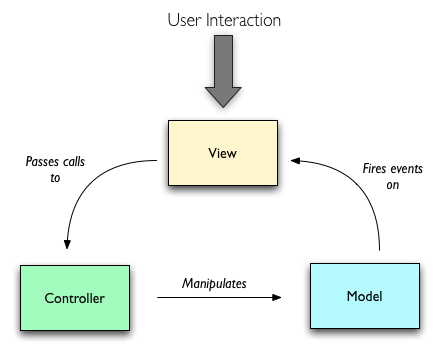
\includegraphics[height = 4cm]{mvc.png}
\end{center}
\end{frame}

\begin{frame}
\frametitle{Project/Site Creation- Part I}
\begin{itemize}
	\item Creating new Project: \hfill \\ \hspace{35pt} .django-admin.py startproject demoproject

	\item Creating new Application: \hfill\\ \hspace{35pt} python manage.py startapp demoapp

	\item Using the built-in web server: \hfill\\ \hspace{35pt} python manage.py runserver
		  
	\item Creating a superuser: \hfill\\ \hspace{35pt} python manage.py createsuperuser
			
			
\end{itemize}
\end{frame}

\begin{frame}
\frametitle{Project/Site Creation- Part II}
\begin{itemize}
  \item Creating Models:  \hfill\\ \hspace{35pt} from django.db import models 

  \item Activating Models:  \hfill\\ \hspace{35pt} python manage.py syncdb

  \item URLs configuration: \hfill\\ \hspace{35pt} from django.conf.urls.defaults import
		  
	\item Creating Views: \hfill\\ \hspace{35pt} from django.http import HttpResponse
			

\end{itemize}
\begin{center}
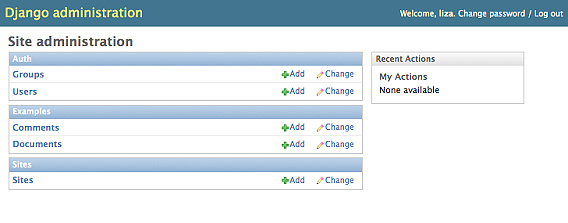
\includegraphics[height = 4cm]{admin.jpg}
\end{center}
\end{frame}

\begin{frame}
\frametitle{Who uses Django?}
\begin{flushleft}
	In conclusion Django is a powerful framework, widely spread in the web development world.
\end{flushleft}
\begin{itemize}
	\item Instagram
	
	\item Mozilla
	
	\item NASA
	
	\item National Geographic, Discovery Channel
	
	\item The Washington Post, NY Times, The Guardian
	
	\item BitBucket
	
	\item PBS (Public Broadcasting Service)

\end{itemize}
\end{frame}


\begin{frame}
\frametitle{Thank you!}
\begin{center}

\includegraphics[height = 4cm]{end.jpg}
\end{center}
\end{frame}


\end{document} 